\documentclass{csbeamer}

\usepackage{dsfont}
\usepackage{amsmath}
\usepackage{amssymb}
\usepackage{algorithm}
\usepackage{algpseudocode}

% Add custom color definitions for Monte Carlo (matching DP pattern)
\definecolor{mcmain}{HTML}{1565C0}
\definecolor{mcaccent}{HTML}{FF6B35}
\definecolor{mclight}{HTML}{42A5F5}
\definecolor{mcsecondary}{HTML}{4CAF50}
\definecolor{mceval}{HTML}{9C27B0}
\definecolor{mcimprove}{HTML}{E91E63}
\definecolor{mcvalue}{HTML}{FF9800}
\definecolor{mcpolicy}{HTML}{795548}
\definecolor{mconpolicy}{HTML}{388E3C}
\definecolor{mcoffpolicy}{HTML}{5D4037}
\definecolor{mcactivity}{HTML}{1976D2}

\university{St. Francis Xavier University}
\department{Department of Computer Science}
\course{CSCI-531 - Reinforcement Learning}
\courseshort{CSCI-531 - RL}
\term{Fall 2025}
\author{Dr. Jean-Alexis Delamer}

\title{Monte Carlo Methods}

\begin{document}

\frame{\titlepage}

% Section: Introduction
\section{Introduction}

\subsection{Beyond Dynamic Programming}

\begin{frame}
    \frametitle{From Model-Based to Model-Free Learning}

    \begin{block}<1->{Dynamic Programming Limitations}
        \begin{itemize}
            \item<1-> Requires \textcolor{mcmain}{\textbf{complete knowledge}} of the environment
            \item<2-> Needs full \textcolor{mcaccent}{\textbf{transition function}} $p(s'|s,a)$
            \item<3-> Often impractical in real-world scenarios
        \end{itemize}
    \end{block}

    \begin{block}<4->{Monte Carlo Solution}
        \begin{center}
            \large{\textcolor{mcaccent}{\textbf{Learn from experience, not models!}}}
        \end{center}
        \begin{itemize}
            \item<5-> Use \textcolor{mceval}{\textbf{episodes}} (complete trajectories)
            \item<6-> Average returns to estimate value functions
            \item<7-> No need for transition probabilities
        \end{itemize}
    \end{block}
\end{frame}

\begin{frame}
    \frametitle{Real-World Motivation}

    \begin{block}<1->{Think About...}
        \textcolor{mcactivity}{\textbf{How would you learn to play a new video game?}}
    \end{block}

    \begin{columns}
        \begin{column}{0.5\textwidth}
            \begin{block}<2->{Traditional DP Approach}
                \begin{itemize}
                    \item<2-> Read the entire manual
                    \item<3-> Study all game mechanics
                    \item<4-> Calculate optimal strategy
                    \item<5-> \textcolor{mcaccent}{\textbf{Then}} start playing
                \end{itemize}
            \end{block}
        \end{column}
        \begin{column}{0.5\textwidth}
            \begin{block}<6->{Monte Carlo Approach}
                \begin{itemize}
                    \item<6-> Jump in and play!
                    \item<7-> Try different actions
                    \item<8-> See what happens
                    \item<9-> \textcolor{mcaccent}{\textbf{Learn from experience}}
                \end{itemize}
            \end{block}
        \end{column}
    \end{columns}

    \begin{block}<10->{Key Insight}
        \textcolor{mcmain}{\textbf{Most real problems are more like the video game scenario!}}
    \end{block}
\end{frame}

\begin{frame}
    \frametitle{The Monte Carlo Approach}

    \begin{block}<1->{Key Insight}
        \begin{center}
            \textcolor{mcmain}{\textbf{Value = Expected Return}}
        \end{center}
        If we can collect many returns from a state, we can \textcolor{mcaccent}{\textbf{average}} them to estimate the true value!
    \end{block}

    \begin{block}<2->{Requirements}
        \begin{itemize}
            \item<2-> Problems must be \textcolor{mceval}{\textbf{episodic}}
            \item<3-> Episodes must eventually \textcolor{mcaccent}{\textbf{terminate}}
            \item<4-> Can still interact with environment (but don't need model)
        \end{itemize}
    \end{block}

    \begin{block}<5->{Important Note}
        \textcolor{mcaccent}{\textbf{Model still needed for interaction, but not for learning!}}
    \end{block}
\end{frame}

\begin{frame}
    \frametitle{Learning Roadmap: Our Journey Through Monte Carlo}

    \begin{block}<1->{Where We're Going}
        \begin{center}
            \begin{tikzpicture}[scale=0.9, every node/.style={font=\small}]
                % Step 1: Prediction
                \node[rectangle, draw=mcmain, fill=mcmain!20, thick, rounded corners=8pt, minimum width=3cm, minimum height=1cm] (pred) at (0,3)
                    {\textbf{1. Prediction}};
                \node[below=3pt of pred, text=mcmain] {\footnotesize Learn $V^\pi(s)$ from episodes};

                % Step 2: Action Values
                \node[rectangle, draw=mcaccent, fill=mcaccent!20, thick, rounded corners=8pt, minimum width=3cm, minimum height=1cm] (action) at (5,3)
                    {\textbf{2. Action Values}};
                \node[below=3pt of action, text=mcaccent] {\footnotesize Why we need $Q^\pi(s,a)$};

                % Step 3: Control
                \node[rectangle, draw=mcsecondary, fill=mcsecondary!20, thick, rounded corners=8pt, minimum width=3cm, minimum height=1cm] (control) at (2.5,0.5)
                    {\textbf{3. Control}};
                \node[below=3pt of control, text=mcsecondary] {\footnotesize Find optimal policies};

                % Arrows
                \draw[->, thick, mcaccent] (pred.east) -- (action.west);
                \draw[->, thick, mcsecondary] (pred.south) -- (control.north west);
                \draw[->, thick, mcsecondary] (action.south) -- (control.north east);

                % Two branches from Control
                \node[rectangle, draw=mconpolicy, fill=mconpolicy!20, thick, rounded corners=6pt, minimum width=2.2cm, minimum height=0.8cm] (onpolicy) at (0.5,-1.5)
                    {\footnotesize On-Policy};
                \node[rectangle, draw=mcoffpolicy, fill=mcoffpolicy!20, thick, rounded corners=6pt, minimum width=2.2cm, minimum height=0.8cm] (offpolicy) at (4.5,-1.5)
                    {\footnotesize Off-Policy};

                \draw[->, thick, mconpolicy] (control.south west) -- (onpolicy.north);
                \draw[->, thick, mcoffpolicy] (control.south east) -- (offpolicy.north);
            \end{tikzpicture}
        \end{center}
    \end{block}


\end{frame}

% Section: Monte Carlo Prediction
\section{Monte Carlo Prediction}

\subsection{Estimating Value Functions}

\begin{frame}
    \frametitle{Monte Carlo Prediction: The Basic Idea}

    \begin{block}<1->{The Process}
        \begin{enumerate}
            \item<1-> Follow policy $\pi$ to generate \textcolor{mcmain}{\textbf{episodes}}
            \item<2-> For each visit to state $s$, record the \textcolor{mcaccent}{\textbf{return}} $G_t$
            \item<3-> Estimate $v_\pi(s)$ as the \textcolor{mcaccent}{\textbf{average}} of all returns from $s$
        \end{enumerate}
    \end{block}

    \begin{block}<4->{Mathematical Foundation}
        \begin{align*}
            v_\pi(s) &= \mathbb{E}_\pi[G_t | S_t = s] \\
            V(s) &\approx \frac{1}{N}\sum_{i=1}^N G_i
        \end{align*}
        where $G_i$ are returns from $N$ visits to state $s$.
    \end{block}

\end{frame}

\begin{frame}
    \frametitle{Episode Collection: The Visual Process}

    \begin{center}
        \begin{tikzpicture}[scale=0.8, every node/.style={font=\footnotesize}]
            % State we're estimating
            \node[circle, draw=mcmain, fill=mcmain!20, thick, minimum size=1.5cm] (state) at (0,3.7) {State $s$};
            \node[below=2pt of state, text=mcmain] {\textbf{What we want: $V^\pi(s)$}};

            % Episode 1
            \node[rectangle, draw=mcaccent, fill=mcaccent!20, rounded corners=4pt, minimum width=3cm, minimum height=0.7cm] (ep1) at (5,5.5) {Episode 1};
            \node[right] at (6.7,5.5) {$G_1 = 8.2$};
            \draw[->, thick, mcaccent] (state.east) -- (ep1.west);

            % Episode 2
            \node[rectangle, draw=mcaccent, fill=mcaccent!20, rounded corners=4pt, minimum width=3cm, minimum height=0.7cm] (ep2) at (5,4.2) {Episode 2};
            \node[right] at (6.7,4.2) {$G_2 = 5.1$};
            \draw[->, thick, mcaccent] (state.east) -- (ep2.west);

            % Episode 3
            \node[rectangle, draw=mcaccent, fill=mcaccent!20, rounded corners=4pt, minimum width=3cm, minimum height=0.7cm] (ep3) at (5,2.9) {Episode 3};
            \node[right] at (6.7,2.9) {$G_3 = 7.8$};
            \draw[->, thick, mcaccent] (state.east) -- (ep3.west);

            % More episodes indicator
            \node at (5,2.3) {\vdots};
            \node at (7.5,2.3) {\vdots};

            % Episode N
            \node[rectangle, draw=mcaccent, fill=mcaccent!20, rounded corners=4pt, minimum width=3cm, minimum height=0.7cm] (epn) at (5,1.5) {Episode N};
            \node[right] at (6.7,1.5) {$G_N = 6.9$};
            \draw[->, thick, mcaccent] (state.east) -- (epn.west);

            % Averaging process
            \node[rectangle, draw=mcsecondary, fill=mcsecondary!20, thick, rounded corners=8pt, minimum width=4cm] (average) at (12,3.7)
                {\textbf{Average All Returns}};
            \node[below=3pt of average, text=mcsecondary] {$V(s) = \frac{G_1 + G_2 + \cdots + G_N}{N}$};

            % Arrow to averaging
            \draw[->, very thick, mcsecondary] (8.5,3.7) -- (average.west);
        \end{tikzpicture}
    \end{center}

    \begin{block}<2->{Key Insight}
        \textcolor{mcmain}{\textbf{More episodes}} $\Rightarrow$ \textcolor{mcsecondary}{\textbf{Better estimate}} of true value!
    \end{block}
\end{frame}

\begin{frame}
    \frametitle{Monte Carlo Prediction: The Basic Idea}

    \begin{block}{Mathematical Foundation}
        \begin{align*}
            v_\pi(s) &= \mathbb{E}_\pi[G_t | S_t = s] \\
            V(s) &\approx \frac{1}{N}\sum_{i=1}^N G_i
        \end{align*}
        where $G_i$ are returns from $N$ visits to state $s$.
    \end{block}

    \begin{block}<2->{Convergence Guarantee}
        As $N \to \infty$, $V(s) \to v_\pi(s)$ by the \textcolor{mceval}{\textbf{Law of Large Numbers}}
    \end{block}
\end{frame}

\begin{frame}
    \frametitle{Concrete Example: Blackjack}

    \textcolor{mcactivity}{\textbf{Consider playing Blackjack with a simple policy:}}
    \begin{itemize}
        \item Hit if hand value < 17
        \item Stand if hand value $\geq$ 17
    \end{itemize}

    \begin{block}<2->{Sample Episodes from State "Hand = 16"}
        \begin{center}
            \begin{tabular}{|c|c|c|}
                \hline
                \textbf{Episode} & \textbf{Outcome} & \textbf{Return} \\
                \hline
                1 & Bust & -1 \\
                2 & Win & +1 \\
                3 & Bust & -1 \\
                4 & Bust & -1 \\
                5 & Lose & -1 \\
                \hline
            \end{tabular}
        \end{center}
    \end{block}

    \begin{block}<3->{Value Estimate}
        $V(\text{Hand}=16) \approx \frac{-1 + 1 + (-1) + (-1) + (-1)}{5} = -0.6$
    \end{block}
\end{frame}

\begin{frame}
    \frametitle{First-Visit vs Every-Visit Monte Carlo}

    \begin{block}<1->{A Key Decision}
        \textcolor{mcactivity}{\textbf{If we visit the same state multiple times in an episode, should we count all visits or just the first one?}}
    \end{block}

    \begin{columns}
        \begin{column}{0.5\textwidth}
            \begin{block}<2->{First-Visit MC}
                \begin{itemize}
                    \item<2-> Only count the \textcolor{mcmain}{\textbf{first}} visit to state $s$ in each episode
                    \item<3-> Simpler to analyze theoretically
                    \item<4-> Guaranteed to converge
                \end{itemize}
            \end{block}
        \end{column}
        \begin{column}{0.5\textwidth}
            \begin{block}<5->{Every-Visit MC}
                \begin{itemize}
                    \item<5-> Count \textcolor{mcaccent}{\textbf{every}} visit to state $s$ in each episode
                    \item<6-> Often converges faster in practice
                    \item<7-> More data per episode
                \end{itemize}
                \end{block}
                \end{column}
                \end{columns}

    \vspace{1em}
    \begin{center}
        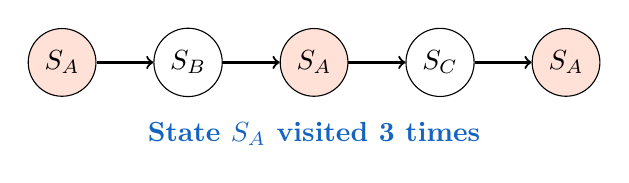
\begin{tikzpicture}[scale=0.8]
            % Episode trajectory
            \node[circle, draw, fill=mcaccent!20] (s1) at (0,0) {$S_A$};
            \node[circle, draw] (s2) at (2,0) {$S_B$};
            \node[circle, draw, fill=mcaccent!20] (s3) at (4,0) {$S_A$};
            \node[circle, draw] (s4) at (6,0) {$S_C$};
            \node[circle, draw, fill=mcaccent!20] (s5) at (8,0) {$S_A$};

            \draw[->, thick] (s1) -- (s2);
            \draw[->, thick] (s2) -- (s3);
            \draw[->, thick] (s3) -- (s4);
            \draw[->, thick] (s4) -- (s5);

            \node[below] at (4,-0.8) {\textcolor{mcmain}{\textbf{State $S_A$ visited 3 times}}};
        \end{tikzpicture}
        \end{center}
        \end{frame}

\begin{frame}
    \frametitle{Why Does This Choice Matter?}

    \begin{block}<1->{Different Perspectives}
        \begin{itemize}
            \item<1-> \textcolor{mcaccent}{\textbf{First-Visit:}} Each episode provides one independent sample per state
            \item<2-> \textcolor{mclight}{\textbf{Every-Visit:}} Each visit provides additional information about the state
        \end{itemize}
        \end{block}

    \begin{block}<3->{Theoretical Implications}
        \begin{itemize}
            \item<3-> \textcolor{mceval}{\textbf{Both are unbiased}} estimators of $v_\pi(s)$
            \item<4-> \textcolor{mcaccent}{\textbf{First-Visit:}} Independent samples, proven convergence
            \item<5-> \textcolor{mclight}{\textbf{Every-Visit:}} Correlated samples, often faster convergence
        \end{itemize}
        \end{block}

    \begin{block}<6->{Practical Guidelines}
        \begin{itemize}
            \item<6-> \textcolor{mcsecondary}{\textbf{Use First-Visit}} for theoretical guarantees and textbook implementations
            \item<7-> \textcolor{mcaccent}{\textbf{Use Every-Visit}} for faster learning and limited computational budget
        \end{itemize}
        \end{block}
    \end{frame}

\begin{frame}
    \frametitle{Interactive Example: Computing Returns}

    \begin{block}<1->{Activity}
        \textcolor{mcactivity}{\textbf{Given this episode with $\gamma = 0.9$:}}
    \end{block}

    \begin{center}
        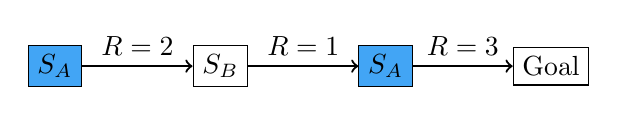
\begin{tikzpicture}[scale=0.7]
            \node[rectangle, draw, fill=mclight] (s1) at (0,0) {$S_A$};
            \node[rectangle, draw] (s2) at (3,0) {$S_B$};
            \node[rectangle, draw, fill=mclight] (s3) at (6,0) {$S_A$};
            \node[rectangle, draw] (s4) at (9,0) {Goal};

            \draw[->, thick] (s1) -- node[above] {$R=2$} (s2);
            \draw[->, thick] (s2) -- node[above] {$R=1$} (s3);
            \draw[->, thick] (s3) -- node[above] {$R=3$} (s4);
        \end{tikzpicture}
    \end{center}

    \begin{block}<2->{Calculate Returns}
        \begin{itemize}
            \item<2-> From first visit to $S_A$: $G_0 = 2 + 0.9 \times 1 + 0.9^2 \times 3 = \textcolor{mcmain}{4.33}$
            \item<3-> From second visit to $S_A$: $G_2 = 3$
        \end{itemize}
    \end{block}

    \begin{block}<4->{Value Estimates}
        \begin{itemize}
            \item<4-> First-Visit MC: $V(S_A) = 4.33$
            \item<5-> Every-Visit MC: $V(S_A) = \frac{4.33 + 3}{2} = \textcolor{mcaccent}{3.67}$
        \end{itemize}
    \end{block}
\end{frame}

\begin{frame}
    \frametitle{Monte Carlo Prediction Algorithm}

    \begin{algorithm}[H]
        \caption{First-Visit Monte Carlo Prediction}
        \begin{algorithmic}[1]
            \State \textbf{Input:} Policy $\pi$, number of episodes $N$
            \State \textbf{Initialize:} $V(s) \in \mathbb{R}$ arbitrarily, $\forall s \in S$; $Returns(s) \leftarrow$ empty list, $\forall s \in S$
            \For{$episode = 1$ to $N$}
                \State Generate episode using $\pi$: $S_0, A_0, R_1, S_1, A_1, R_2, \ldots, S_{T-1}, A_{T-1}, R_T$
                \State $G \leftarrow 0$
                \For{$t = T-1, T-2, \ldots, 0$}
                    \State $G \leftarrow \gamma G + R_{t+1}$
                    \If{$S_t \notin \{S_0, S_1, \ldots, S_{t-1}\}$}
                        \State Append $G$ to $Returns(S_t)$
                        \State $V(S_t) \leftarrow$ average$(Returns(S_t))$
                    \EndIf
                \EndFor
            \EndFor
        \end{algorithmic}
    \end{algorithm}
\end{frame}

\begin{frame}
    \frametitle{Common Mistakes and Pitfalls}

    \begin{block}<1->{Pitfall \#1: Wrong Direction}
        \textcolor{mcaccent}{\textbf{Why do we go backwards through the episode?}}
        \begin{itemize}
            \item<2-> Returns are calculated from \textcolor{mcmain}{\textbf{future rewards}}
            \item<3-> Working backwards ensures we have all future rewards available
            \item<4-> More efficient than recalculating from scratch each time
        \end{itemize}
    \end{block}
\end{frame}

\begin{frame}
    \frametitle{Common Mistakes and Pitfalls}

    \begin{block}<1->{Pitfall \#2: Insufficient Episodes}
        \textcolor{mcaccent}{\textbf{How many episodes do we need?}}
        \begin{itemize}
            \item<2-> Depends on state space size and variance
            \item<3-> Start with \textcolor{mcsecondary}{\textbf{1000+ episodes}} for simple problems
            \item<4-> Monitor convergence of value estimates
        \end{itemize}
    \end{block}
\end{frame}

\begin{frame}
    \frametitle{From Prediction to Control: What's Missing?}

    \begin{block}<1->{What We've Learned So Far}
        \begin{itemize}
            \item<1-> We can estimate \textcolor{mcmain}{\textbf{state values}} $V^\pi(s)$ using episodes
            \item<2-> We know how good each state is under policy $\pi$
            \item<3-> We have a working Monte Carlo prediction algorithm
        \end{itemize}
    \end{block}

    \begin{block}<4->{The Next Challenge: Finding Better Policies}
        \textcolor{mcactivity}{\textbf{Question:}} If we know $V^\pi(s)$ for all states, can we immediately find a better policy?
    \end{block}

    \begin{block}<5->{The Problem}
        \begin{itemize}
            \item<5-> In DP: $\pi'(s) = \arg\max_a \sum_{s'} p(s'|s,a)[r + \gamma V^\pi(s')]$
            \item<6-> \textcolor{mcaccent}{\textbf{But we don't know}} $p(s'|s,a)$ in model-free settings!
            \item<7-> We need a different approach...
        \end{itemize}
    \end{block}
\end{frame}

% Section: Monte Carlo Estimation of Action Values
\section{Action Value Estimation}

\subsection{From State Values to Action Values}

\begin{frame}
    \frametitle{Why Action Values in Model-Free Settings?}

    \begin{block}<1->{Discussion Question}
        If we have perfect state values $V^*(s)$, can we immediately determine the optimal policy without knowing the model?
    \end{block}

    \begin{columns}
        \begin{column}{0.5\textwidth}
            \begin{block}<2->{The Problem with State Values}
                \begin{itemize}
                    \item<2-> In DP: $\pi(s) = \arg\max_a \sum_{s'} p(s'|s,a)[r + \gamma V(s')]$
                    \item<3-> \textcolor{mcmain}{\textbf{Requires}} transition probabilities $p(s'|s,a)$
                    \item<4-> Not available in model-free settings!
                \end{itemize}
            \end{block}
        \end{column}

        \begin{column}{0.5\textwidth}
            \begin{center}
                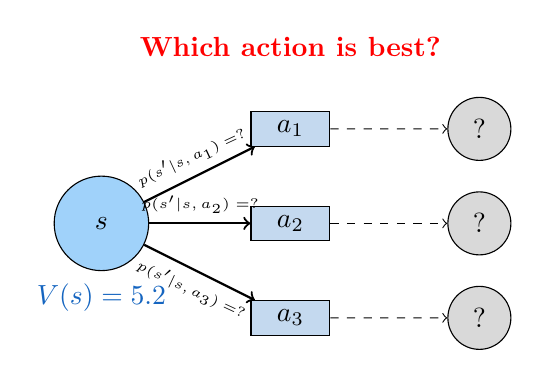
\begin{tikzpicture}[scale=0.8]
                    % Current state
                    \node[circle, draw, fill=mclight!50, minimum size=1.2cm] (s) at (0,0) {$s$};
                    \node[below] at (0,-0.8) {\textcolor{mcmain}{$V(s) = 5.2$}};

                    % Actions
                    \node[rectangle, draw, fill=mcmain!25, minimum width=1cm] (a1) at (3,1.5) {$a_1$};
                    \node[rectangle, draw, fill=mcmain!25, minimum width=1cm] (a2) at (3,0) {$a_2$};
                    \node[rectangle, draw, fill=mcmain!25, minimum width=1cm] (a3) at (3,-1.5) {$a_3$};

                    % Future states (with question marks)
                    \node[circle, draw, fill=gray!30, minimum size=0.8cm] (s1) at (6,1.5) {?};
                    \node[circle, draw, fill=gray!30, minimum size=0.8cm] (s2) at (6,0) {?};
                    \node[circle, draw, fill=gray!30, minimum size=0.8cm] (s3) at (6,-1.5) {?};

                    % Arrows with question marks for probabilities
                    \draw[->, thick] (s) -- node[above, rotate=25] {\tiny $p(s'|s, a_1) = ?$} (a1);
                    \draw[->, thick] (s) -- node[above] {\tiny $p(s'|s,a_2) = ?$} (a2);
                    \draw[->, thick] (s) -- node[below, rotate=-25] {\tiny $p(s'|s,a_3) = ?$} (a3);

                    \draw[->, dashed] (a1) -- (s1);
                    \draw[->, dashed] (a2) -- (s2);
                    \draw[->, dashed] (a3) -- (s3);

                    % Question mark for best action
                    \node[above] at (3,2.5) {\textcolor{red}{\textbf{Which action is best?}}};
                \end{tikzpicture}
            \end{center}

        \end{column}
    \end{columns}
\end{frame}

\begin{frame}
    \frametitle{The Fundamental Problem: State Values Aren't Enough}

    \begin{block}<1->{Imagine This Scenario}
        \textcolor{mcactivity}{\textbf{You're playing a game and reach this state:}}
        \begin{center}
            You have \textcolor{mcmain}{\textbf{perfect knowledge}} that being here is worth +5.2 points on average
        \end{center}
    \end{block}

    \begin{block}<2->{The Question}
        \textcolor{mcaccent}{\textbf{What should you do next?}}
    \end{block}

    \begin{columns}
        \begin{column}{0.5\textwidth}
            \begin{block}<3->{Available Actions}
                \begin{itemize}
                    \item<3-> \textcolor{mclight}{\textbf{Action A}}: Move left
                    \item<4-> \textcolor{mclight}{\textbf{Action B}}: Move right
                    \item<5-> \textcolor{mclight}{\textbf{Action C}}: Jump
                \end{itemize}
            \end{block}
        \end{column}
        \begin{column}{0.5\textwidth}
            \begin{block}<6->{The Problem}
                \begin{itemize}
                    \item<6-> You know the state is good
                    \item<7-> But \textcolor{mcaccent}{\textbf{which action}} leads to the best outcome?
                    \item<8-> State value doesn't tell you!
                \end{itemize}
            \end{block}
        \end{column}
    \end{columns}
\end{frame}

\begin{frame}
    \frametitle{Action Values: The Missing Piece}

    \begin{block}<1->{What We Really Need}
        \begin{center}
            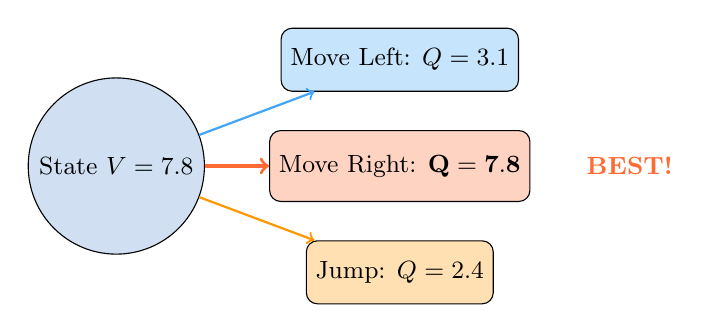
\begin{tikzpicture}[scale=0.9, every node/.style={font=\small}]
                % Current state
                \node[circle, draw, fill=mcmain!20, minimum size=1.5cm] (s) at (0,0) {State $V=7.8$};

                % Action values with clear differences
                \node[rectangle, draw, fill=mclight!30, minimum width=2.2cm, minimum height=0.8cm, rounded corners] (q1) at (4,1.5) {Move Left: $Q=3.1$};
                \node[rectangle, draw, fill=mcaccent!30, minimum width=2.2cm, minimum height=0.9cm, rounded corners] (q2) at (4,0) {Move Right: $\mathbf{Q=7.8}$};
                \node[rectangle, draw, fill=mcvalue!30, minimum width=2.2cm, minimum height=0.8cm, rounded corners] (q3) at (4,-1.5) {Jump: $Q=2.4$};

                % Arrows showing choice
                \draw[->, thick, mclight] (s) -- (q1);
                \draw[->, very thick, mcaccent] (s) -- (q2);
                \draw[->, thick, mcvalue] (s) -- (q3);

                % Clear winner
                \node[right, text=mcaccent] at (6.5,0) {\textbf{BEST!}};
            \end{tikzpicture}
        \end{center}
    \end{block}

    \begin{block}<2->{Now We Can Decide!}
        \begin{itemize}
            \item<2-> \textcolor{mcaccent}{\textbf{Move Right}} has highest Q-value (7.8)
            \item<3-> \textcolor{mcsecondary}{\textbf{Simple policy}}: $\pi(s) = \arg\max_a Q(s,a)$
        \end{itemize}
    \end{block}
\end{frame}

\begin{frame}
    \frametitle{Why This Changes Everything}

    \begin{block}<1->{The Key Insight}
        \textcolor{mcactivity}{\textbf{Action values give us direct decision-making power!}}
    \end{block}

    \begin{block}<2->{The Difference}
        \begin{itemize}
            \item<2-> \textcolor{mclight}{\textbf{State values $V(s)$}}: Know how good states are, still need model for decisions
            \item<3-> \textcolor{mcaccent}{\textbf{Action values $Q(s,a)$}}: Know how good actions are, can decide immediately
            \item<4-> \textcolor{mcsecondary}{\textbf{Result}}: Model-free decision making!
        \end{itemize}
    \end{block}

    \begin{block}<5->{New Challenge}
        \textcolor{mcaccent}{\textbf{Exploration Problem:}} All actions must be visited to get good estimates!
    \end{block}
\end{frame}

\begin{frame}
    \frametitle{The Exploration Problem}

    \begin{center}
        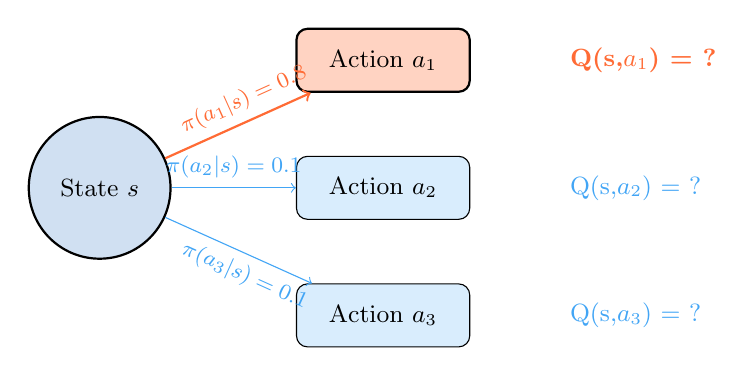
\begin{tikzpicture}[scale=0.9, every node/.style={font=\small}]
            % State
            \node[circle, draw, fill=mcmain!20, minimum size=1.8cm, thick] (state) at (0,0) {State $s$};

            % Actions with better spacing and consistent styling
            \node[rectangle, draw, fill=mcaccent!30, minimum width=2.2cm, minimum height=0.8cm, rounded corners, thick] (a1) at (4,1.8) {Action $a_1$};
            \node[rectangle, draw, fill=mclight!20, minimum width=2.2cm, minimum height=0.8cm, rounded corners] (a2) at (4,0) {Action $a_2$};
            \node[rectangle, draw, fill=mclight!20, minimum width=2.2cm, minimum height=0.8cm, rounded corners] (a3) at (4,-1.8) {Action $a_3$};

            % Arrows with better positioned labels
            \draw[->, thick, mcaccent] (state) -- node[above, sloped, pos=0.6] {\footnotesize $\pi(a_1|s) = 0.8$} (a1);
            \draw[->, mclight] (state) -- node[above, pos=0.5] {\footnotesize $\pi(a_2|s) = 0.1$} (a2);
            \draw[->, mclight] (state) -- node[below, sloped, pos=0.6] {\footnotesize $\pi(a_3|s) = 0.1$} (a3);

            % Q-value estimates with better alignment
            \node[right, align=left] at (6.5,1.8) {\textcolor{mcaccent}{\textbf{Q(s,$a_1$) = ?}}};
            \node[right, align=left] at (6.5,0) {\textcolor{mclight}{Q(s,$a_2$) = ?}};
            \node[right, align=left] at (6.5,-1.8) {\textcolor{mclight}{Q(s,$a_3$) = ?}};
        \end{tikzpicture}
    \end{center}

    \begin{block}<2->{The Dilemma}
        \begin{itemize}
            \item<2-> \textcolor{mcsecondary}{\textbf{Greedy action}} gets lots of data → good estimate
            \item<3-> \textcolor{mcaccent}{\textbf{Other actions}} get little data → poor estimates
            \item<4-> How do we know if unexplored actions are actually better?
        \end{itemize}
    \end{block}
    \end{frame}

\begin{frame}
    \frametitle{Solutions to the Exploration Problem}

    \begin{block}<1->{Option 1: Exploring Starts}
        \begin{itemize}
            \item<1-> Every episode starts with random state-action pair
            \item<2-> Guarantees all $(s,a)$ pairs are visited
            \item<3-> \textcolor{mcaccent}{\textbf{Problem:}} Often not practical in real applications
        \end{itemize}
    \end{block}

    \begin{block}<4->{Option 2: Soft Policies (Our Focus)}
        \begin{itemize}
            \item<4-> Maintain \textcolor{mcsecondary}{\textbf{non-zero probability}} for all actions
            \item<5-> Balance exploration and exploitation
            \item<6-> Example: \textcolor{mceval}{\textbf{$\epsilon$-greedy policies}}
        \end{itemize}
    \end{block}
\end{frame}

% Section: Monte Carlo Control
\section{Monte Carlo Control}

\subsection{On-Policy Methods}

\begin{frame}
    \frametitle{On-Policy Monte Carlo Control}

    \begin{block}<1->{The Approach}
        \begin{itemize}
            \item<1-> Learn the value of the \textcolor{mconpolicy}{\textbf{same policy}} we're following
            \item<2-> Use \textcolor{mcaccent}{\textbf{$\epsilon$-greedy}} policy for exploration
            \item<3-> Gradually improve policy based on learned action values
        \end{itemize}
        \end{block}

    \begin{block}<4->{$\epsilon$-Greedy Policy}
        \begin{align*}
            \pi(a|s) = \begin{cases}
                1 - \epsilon + \frac{\epsilon}{|A|} & \text{if } a = \arg\max_a Q(s,a) \\
                \frac{\epsilon}{|A|} & \text{otherwise}
            \end{cases}
        \end{align*}
    \end{block}
 \end{frame}

 \begin{frame}
     \frametitle{On-Policy Monte Carlo Control}

     \begin{block}<1->{$\epsilon$-Greedy Policy}
         \begin{align*}
             \pi(a|s) = \begin{cases}
                 1 - \epsilon + \frac{\epsilon}{|A|} & \text{if } a = \arg\max_a Q(s,a) \\
                 \frac{\epsilon}{|A|} & \text{otherwise}
             \end{cases}
         \end{align*}
     \end{block}

     \begin{block}<2->{Key Properties}
         \begin{itemize}
             \item<2-> \textcolor{mcsecondary}{\textbf{Soft policy:}} All actions have non-zero probability
             \item<3-> \textcolor{mceval}{\textbf{Improvement guarantee:}} Any $\epsilon$-greedy policy w.r.t. $Q_\pi$ is better than $\pi$
         \end{itemize}
     \end{block}
  \end{frame}

\begin{frame}
    \frametitle{$\epsilon$-Greedy Policy Example}
    \begin{block}<1->{Interactive Example}
        State $s$ has 3 actions with $\epsilon = 0.2$:
        \begin{center}
            $Q(s,a_1) = 5$, $Q(s,a_2) = 3$, $Q(s,a_3) = 1$
        \end{center}
    \end{block}

    \begin{block}<2->{Calculate $\epsilon$-greedy probabilities:}
        \begin{itemize}
            \item<2-> Best action: $a_1$ (greedy action)
            \item<3-> $\pi(a_1|s) = 1 - 0.2 + \frac{0.2}{3} = 0.8 + 0.067 = \textcolor{mcsecondary}{0.867}$
            \item<4-> $\pi(a_2|s) = \frac{0.2}{3} = \textcolor{mcaccent}{0.067}$
            \item<5-> $\pi(a_3|s) = \frac{0.2}{3} = \textcolor{mcaccent}{0.067}$
        \end{itemize}
        \end{block}

    \begin{center}<7->
        \textcolor{mcactivity}{\textbf{What happens as we learn and $Q$ values change?}}
    \end{center}
    \end{frame}

\begin{frame}
    \begin{algorithm}[H]
        \caption{On-Policy First-Visit MC Control}
        \begin{algorithmic}[1]
            \State \textbf{Initialize:} $Q(s,a) \in \mathbb{R}$ arbitrarily, $\forall s \in S, a \in A$
            \State \textbf{Initialize:} $\pi \leftarrow$ arbitrary $\epsilon$-soft policy; $Returns(s,a) \leftarrow$ empty list, $\forall s \in S, a \in A$
            \For{each episode}
                \State Generate episode using $\pi$: $S_0, A_0, R_1, \ldots, S_{T-1}, A_{T-1}, R_T$
                \State $G \leftarrow 0$
                \For{$t = T-1, T-2, \ldots, 0$}
                    \State $G \leftarrow \gamma G + R_{t+1}$
                    \If{$(S_t, A_t) \notin \{(S_0, A_0), \ldots, (S_{t-1}, A_{t-1})\}$}
                        \State Append $G$ to $Returns(S_t, A_t)$
                        \State $Q(S_t, A_t) \leftarrow$ average$(Returns(S_t, A_t))$
                        \State $A^* \leftarrow \arg\max_a Q(S_t, a)$
                        \For{all $a \in A$}
                            \State $\pi(a|S_t) \leftarrow \begin{cases}
                                1 - \epsilon + \frac{\epsilon}{|A|} & \text{if } a = A^* \\
                                \frac{\epsilon}{|A|} & \text{otherwise}
                            \end{cases}$
                        \EndFor
                    \EndIf
                \EndFor
            \EndFor
        \end{algorithmic}
    \end{algorithm}
\end{frame}

\begin{frame}
    \frametitle{Concrete Example Part 1: Q-Value Update}

    \begin{block}<1->{Current Situation}
        \textcolor{mcactivity}{\textbf{State: Hand = 16, Actions: Hit or Stand}}
        \begin{center}
        \begin{tabular}{|c|c|c|}
        \hline
        \textbf{Action} & \textbf{Current Q-value} & \textbf{Returns History} \\
        \hline
        Hit & $Q(16, \text{Hit}) = 0.2$ & $[0.1, 0.3]$ \\
        Stand & $Q(16, \text{Stand}) = 0.5$ & $[0.5]$ \\
        \hline
        \end{tabular}
        \end{center}
    \end{block}

    \begin{block}<2->{Episode Update}
        \begin{itemize}
            \item<2-> Chose \textcolor{mcaccent}{\textbf{Hit}}, got return $G = 0.7$
            \item<3-> $Returns(16, \text{Hit}) = [0.1, 0.3, \textcolor{mcaccent}{0.7}]$
            \item<4-> $Q(16, \text{Hit}) = \frac{0.1 + 0.3 + 0.7}{3} = \textcolor{mcaccent}{0.37}$
            \item<5-> \textcolor{mcsecondary}{\textbf{Result:}} Hit improved from 0.2 to 0.37, Stand stays 0.5
        \end{itemize}
    \end{block}
\end{frame}

\begin{frame}
    \frametitle{Concrete Example Part 2: Policy Update}

    \begin{block}<1->{Current Q-Values}
        \begin{center}
        \begin{tabular}{|c|c|}
        \hline
        \textbf{Action} & \textbf{Q-value} \\
        \hline
        Hit & $Q(16, \text{Hit}) = 0.37$ \\
        Stand & $Q(16, \text{Stand}) = 0.5$ \\
        \hline
        \end{tabular}
        \end{center}
    \end{block}

    \begin{block}<2->{Policy Update with $\epsilon = 0.1$:}
        \begin{itemize}
            \item<2-> Best action: $\arg\max \{0.37, 0.5\} = \textcolor{mcsecondary}{\text{Stand}}$
            \item<3-> $\pi(\text{Stand}|16) = 1 - 0.1 + \frac{0.1}{2} = \textcolor{mcsecondary}{0.95}$
            \item<4-> $\pi(\text{Hit}|16) = \frac{0.1}{2} = 0.05$
        \end{itemize}
    \end{block}

\end{frame}

\subsection{Off-Policy Methods}

\begin{frame}
    \frametitle{Off-Policy Monte Carlo: Motivation}

    \begin{block}<1->{Limitation of On-Policy Methods}
        \textcolor{mcactivity}{\textbf{What's the best policy on-policy MC can find?}}
    \end{block}

    \begin{block}<2->{The Issue}
        \begin{itemize}
            \item<2-> Can only find best policy among \textcolor{mcaccent}{\textbf{$\epsilon$-soft policies}}
            \item<3-> Always includes some exploration (suboptimal actions)
            \item<4-> Cannot learn truly \textcolor{mcmain}{\textbf{optimal deterministic}} policy
        \end{itemize}
    \end{block}

    \begin{block}<5->{Off-Policy Solution}
        \begin{itemize}
            \item<5-> Use two policies:
            \begin{itemize}
                \item<6-> Target Policy $\pi$: The policy we want to learn (can be deterministic)
                \item<7-> Behavior Policy $b$: The policy we follow for exploration
            \end{itemize}
            \item<8-> Learn about $\pi$ using data generated by $b$
        \end{itemize}
        \end{block}
        \end{frame}

\begin{frame}
    \frametitle{Off-Policy Concept Visualization}

    \begin{center}
        \begin{tikzpicture}[scale=0.8, every node/.style={font=\small}]
            % Target policy - rounded rectangle
            \node[rectangle, draw=mcsecondary, fill=mcsecondary!20, thick, rounded corners=12pt, minimum width=4cm, minimum height=1.2cm] (target) at (0,3)
                {\textbf{Target Policy $\pi$}};
            \node[below=3pt of target, text=mcsecondary] {\footnotesize Greedy/Optimal - What we want to learn};

            % Behavior policy - rounded rectangle
            \node[rectangle, draw=mceval, fill=mceval!20, thick, rounded corners=12pt, minimum width=4cm, minimum height=1.2cm] (behavior) at (0,0)
                {\textbf{Behavior Policy $b$}};
            \node[below=3pt of behavior, text=mceval] {\footnotesize $\epsilon$-greedy - What we follow};

            % Episodes - distinct rounded rectangle
            \node[rectangle, draw=mcaccent, fill=mcaccent!20, thick, rounded corners=8pt, minimum width=3.5cm, minimum height=1.1cm] (episodes) at (7,1.5)
                {\textbf{Episodes}};
            \node[below=3pt of episodes, text=mcaccent] {\footnotesize Generated by $b$};

            % Clean arrows with better spacing
            \draw[->, thick, mceval] (behavior.east) -- node[below] {\footnotesize Generate} (episodes.west);
            \draw[->, thick, dashed, mcsecondary] (episodes.north west) -- node[above] {\footnotesize Learn about} (target.east);
        \end{tikzpicture}
    \end{center}

    \begin{block}<2->{Coverage Assumption}
        $\pi(a|s) > 0 \Rightarrow b(a|s) > 0$ for all $s, a$

        \textcolor{mcactivity}{\textbf{Why is this assumption crucial?}}
    \end{block}
    \end{frame}

\begin{frame}
    \frametitle{Simple Analogy: YouTube Gaming Videos}

    \begin{block}<1->{Imagine You Want to Know...}
        \textcolor{mcactivity}{\textbf{How good are speedrunners at this game?}}
    \end{block}

    \begin{block}<2->{The Problem}
        \begin{itemize}
            \item<2-> You mostly have gameplay videos from \textcolor{mcaccent}{\textbf{casual players}} (not speedrunners)
            \item<3-> Casual players use "safe strategy" 80\% of the time
            \item<4-> Speedrunners would use "risky strategy" 80\% of the time
            \item<5-> How do you estimate speedrunner performance?
        \end{itemize}
    \end{block}

    \begin{block}<6->{The Solution: Weight the Gameplay}
        \begin{itemize}
            \item<6-> Casual player videos are \textcolor{mcaccent}{\textbf{over-represented}} for safe moves
            \item<7-> Weight risky moves by $\frac{0.80}{0.20} = 4.0$
            \item<8-> This "up-weights" the rare risky gameplay we want to learn about
        \end{itemize}
    \end{block}
\end{frame}

\begin{frame}
    \frametitle{From Gaming to Reinforcement Learning}

    \begin{block}<1->{The Connection}
        \begin{center}
        \begin{tabular}{|c|c|}
        \hline
        \textbf{YouTube Gaming} & \textbf{RL Off-Policy} \\
        \hline
        Casual players & Behavior policy $b$ \\
        Speedrunners & Target policy $\pi$ \\
        Strategy choices & Episode actions \\
        Game scores & Episode returns \\
        Weight = 0.80/0.20 & Weight = $\pi(a|s)/b(a|s)$ \\
        \hline
        \end{tabular}
        \end{center}
    \end{block}

    \begin{block}<2->{Key Insight}
        \textcolor{mcsecondary}{\textbf{When gameplay comes from the "wrong" player type, we reweight it to match the strategy we want to learn!}}
    \end{block}
\end{frame}

\begin{frame}
    \frametitle{Importance Sampling Intuition}

    \begin{block}<1->{The Problem}
        \textcolor{mcactivity}{\textbf{We have episodes from policy $b$, but want to learn about policy $\pi$. How do we account for the difference?}}
    \end{block}

    \begin{block}<2->{Intuitive Example}
        \begin{itemize}
            \item<2-> Suppose $b$ takes action $a_1$ with probability 0.8
            \item<3-> But $\pi$ would take $a_1$ with probability 0.2
            \item<4-> Episodes with $a_1$ are \textcolor{mcaccent}{\textbf{over-represented}} in our data
            \item<5-> We need to \textcolor{mcsecondary}{\textbf{down-weight}} these episodes
        \end{itemize}
        \end{block}

    \begin{block}<6->{The Solution: Importance Sampling}
        \begin{center}
            \textcolor{mcmain}{\textbf{Weight each episode by the ratio of its probability under $\pi$ vs $b$}}
        \end{center}
        \end{block}
        \end{frame}

\begin{frame}
    \frametitle{Importance Sampling Mathematics}

    \begin{block}<1->{Importance Sampling Ratio}
        \begin{align*}
            \rho_{t:T-1} &= \frac{\text{Prob of trajectory under } \pi}{\text{Prob of trajectory under } b} \\
            &= \frac{\prod_{k=t}^{T-1} \pi(A_k|S_k) p(S_{k+1}|S_k, A_k)}{\prod_{k=t}^{T-1} b(A_k|S_k) p(S_{k+1}|S_k, A_k)} \\
            &= \prod_{k=t}^{T-1} \frac{\pi(A_k|S_k)}{b(A_k|S_k)}
        \end{align*}
    \end{block}

    \begin{block}<2->{Key Insight}
        \textcolor{mcsecondary}{\textbf{Transition probabilities cancel out!}} Only depends on policies.
    \end{block}

    \end{frame}

\begin{frame}
    \frametitle{Importance Sampling: Numerical Example}

    \begin{block}<1->{Episode Trajectory}
        \textcolor{mcactivity}{\textbf{Episode: $S_0 \xrightarrow{A_0} S_1 \xrightarrow{A_1} S_2$}}
    \end{block}

    \begin{block}<2->{Policy Probabilities}
        \begin{itemize}
            \item<2-> At $S_0$: $\pi(A_0|S_0) = 0.1$, $b(A_0|S_0) = 0.3$
            \item<3-> At $S_1$: $\pi(A_1|S_1) = 0.8$, $b(A_1|S_1) = 0.4$
        \end{itemize}
    \end{block}

    \begin{block}<4->{Importance Sampling Ratio}
        \begin{align*}
            \rho &= \frac{\pi(A_0|S_0)}{b(A_0|S_0)} \times \frac{\pi(A_1|S_1)}{b(A_1|S_1)} \\
            &= \frac{0.1}{0.3} \times \frac{0.8}{0.4} = \frac{1}{3} \times 2 = \frac{2}{3}
        \end{align*}
    \end{block}
    \end{frame}

\begin{frame}
    \begin{algorithm}[H]
        \caption{Off-Policy Monte Carlo Prediction}
        \begin{algorithmic}[1]
            \State \textbf{Initialize:} $Q(s,a) \in \mathbb{R}$ arbitrarily, $\forall s \in S, a \in A$
            \State \textbf{Initialize:} $C(s,a) \leftarrow 0$, $\forall s \in S, a \in A$
            \For{each episode}
                \State $b \leftarrow$ any policy with coverage of $\pi$
                \State Generate episode using $b$: $S_0, A_0, R_1, \ldots, S_{T-1}, A_{T-1}, R_T$
                \State $G \leftarrow 0$, $W \leftarrow 1$
                \For{$t = T-1, T-2, \ldots, 0$ and $W \neq 0$}
                    \State $G \leftarrow \gamma G + R_{t+1}$
                    \State $C(S_t, A_t) \leftarrow C(S_t, A_t) + W$
                    \State $Q(S_t, A_t) \leftarrow Q(S_t, A_t) + \frac{W}{C(S_t, A_t)}[G - Q(S_t, A_t)]$
                    \State $W \leftarrow W \cdot \frac{\pi(A_t|S_t)}{b(A_t|S_t)}$
                \EndFor
            \EndFor
        \end{algorithmic}
    \end{algorithm}

    \end{frame}

\begin{frame}
    \frametitle{Weighted Importance Sampling: Key Features}

    \begin{block}<1->{Implementation Details}
        \begin{itemize}
            \item<1-> Uses \textcolor{mcaccent}{\textbf{incremental implementation}} with weighted average
            \item<2-> Stops if $W = 0$ (trajectory impossible under target policy)
        \end{itemize}
    \end{block}

    \begin{block}<3->{Why This Matters}
        \begin{itemize}
            \item<3-> \textcolor{mcsecondary}{\textbf{Efficiency}}: No need to store all returns
            \item<4-> \textcolor{mceval}{\textbf{Robustness}}: Handles impossible trajectories gracefully
            \item<5-> \textcolor{mcmain}{\textbf{Convergence}}: Weighted averaging often has better properties
        \end{itemize}
    \end{block}
    \end{frame}

\begin{frame}
    \begin{algorithm}[H]
        \caption{Off-Policy Monte Carlo Control}
        \begin{algorithmic}[1]
            \State \textbf{Initialize:} $\pi(s) \leftarrow \arg\max_a Q(s,a)$ (greedy policy)
            \For{each episode}
                \State $b \leftarrow$ any policy with coverage of $\pi$
                \State Generate episode using $b$: $S_0, A_0, R_1, \ldots, S_{T-1}, A_{T-1}, R_T$
                \State $G \leftarrow 0$, $W \leftarrow 1$
                \For{$t = T-1, T-2, \ldots, 0$ and $W \neq 0$}
                    \State $G \leftarrow \gamma G + R_{t+1}$
                    \State $C(S_t, A_t) \leftarrow C(S_t, A_t) + W$
                    \State $Q(S_t, A_t) \leftarrow Q(S_t, A_t) + \frac{W}{C(S_t, A_t)}[G - Q(S_t, A_t)]$
                    \State $\pi(S_t) \leftarrow \arg\max_a Q(S_t, a)$
                    \If{$A_t \neq \pi(S_t)$}
                        \State \textbf{break} (exit inner loop)
                    \EndIf
                    \State $W \leftarrow W \cdot \frac{1}{b(A_t|S_t)}$
                \EndFor
            \EndFor
        \end{algorithmic}
    \end{algorithm}
    \end{frame}

% Learning Progress Visualization
\begin{frame}
    \frametitle{Learning Progress: How Monte Carlo Converges}

    \begin{block}<1->{What Does Learning Look Like?}
        \textcolor{mcactivity}{\textbf{Let's visualize how our value estimates improve over time}}
    \end{block}

    \begin{center}
        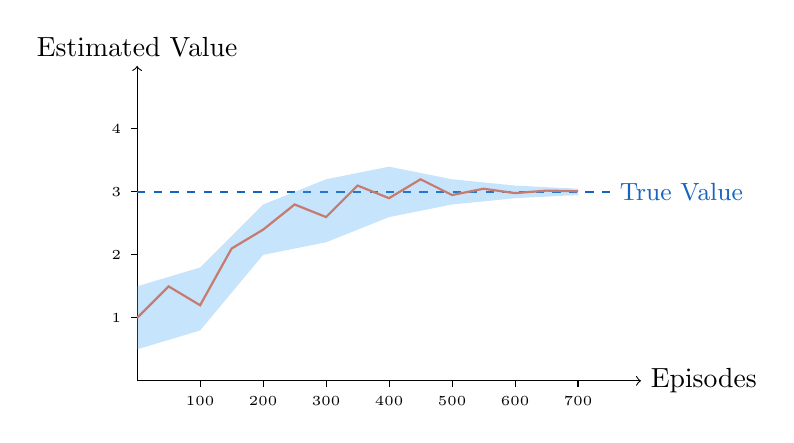
\begin{tikzpicture}[scale=0.8]
            % Axes
            \draw[->] (0,0) -- (8,0) node[right] {Episodes};
            \draw[->] (0,0) -- (0,5) node[above] {Estimated Value};

            % True value line
            \draw[thick, mcmain, dashed] (0,3) -- (7.5,3) node[right] {\small True Value};

            % Learning curve with variance
            \draw[thick, mcaccent]
                (0,1) -- (0.5,1.5) -- (1,1.2) -- (1.5,2.1) -- (2,2.4) --
                (2.5,2.8) -- (3,2.6) -- (3.5,3.1) -- (4,2.9) -- (4.5,3.2) --
                (5,2.95) -- (5.5,3.05) -- (6,2.98) -- (6.5,3.02) -- (7,3.01);

            % Confidence band
            \fill[mclight, opacity=0.3]
                (0,0.5) -- (1,0.8) -- (2,2.0) -- (3,2.2) -- (4,2.6) -- (5,2.8) -- (6,2.9) -- (7,2.95) --
                (7,3.05) -- (6,3.1) -- (5,3.2) -- (4,3.4) -- (3,3.2) -- (2,2.8) -- (1,1.8) -- (0,1.5) -- cycle;

            % Episode markers
            \foreach \x in {1,2,3,4,5,6,7}
                \draw (\x,0) -- (\x,-0.1) node[below] {\tiny \x 00};

            % Value markers
            \foreach \y in {1,2,3,4}
                \draw (0,\y) -- (-0.1,\y) node[left] {\tiny \y};
        \end{tikzpicture}
    \end{center}

    \begin{block}<2->{Key Observations}
        \begin{itemize}
            \item<2-> \textcolor{mcaccent}{\textbf{High variance}} early in learning (few samples)
            \item<3-> Estimates \textcolor{mcmain}{\textbf{converge}} to true value with more episodes
            \item<4-> \textcolor{mcsecondary}{\textbf{Sample complexity}} depends on environment and policy
        \end{itemize}
    \end{block}
\end{frame}

\begin{frame}
    \frametitle{Practical Learning Considerations}

    \begin{block}<1->{What Affects Convergence Speed?}
        \begin{columns}
            \begin{column}{0.5\textwidth}
                \textcolor{mcaccent}{\textbf{Faster Convergence:}}
                \begin{itemize}
                    \item<2-> Low variance returns
                    \item<3-> Frequent state visits
                    \item<4-> Shorter episodes
                    \item<5-> Deterministic rewards
                \end{itemize}
            \end{column}
            \begin{column}{0.5\textwidth}
                \textcolor{mcmain}{\textbf{Slower Convergence:}}
                \begin{itemize}
                    \item<6-> High variance returns
                    \item<7-> Rare state visits
                    \item<8-> Long episodes
                    \item<9-> Stochastic environments
                \end{itemize}
            \end{column}
        \end{columns}
    \end{block}
\end{frame}

% Control Flow Diagram
\begin{frame}
    \frametitle{Monte Carlo Control: The Complete Loop}

    \begin{block}<1->{The Big Picture}
        \textcolor{mcactivity}{\textbf{How do all the pieces fit together?}}
    \end{block}

    \begin{center}
        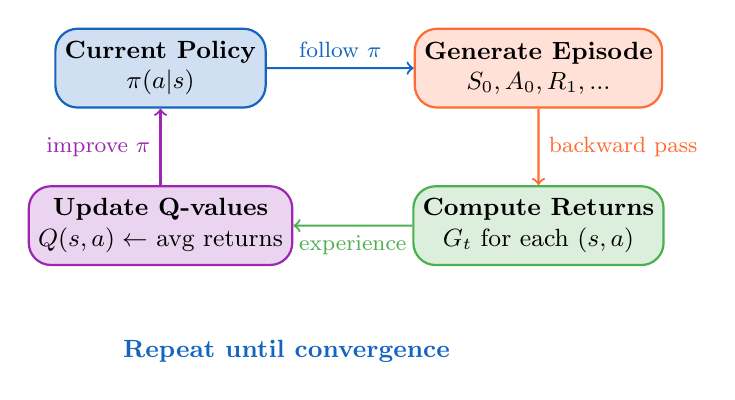
\begin{tikzpicture}[scale=0.8, every node/.style={font=\small}]
            % Main loop components
            \node[rectangle, draw=mcmain, fill=mcmain!20, thick, rounded corners=8pt, minimum width=2.5cm, minimum height=1cm, align=center] (policy) at (0,4)
                {\textbf{Current Policy} \\ $\pi(a|s)$};

            \node[rectangle, draw=mcaccent, fill=mcaccent!20, thick, rounded corners=8pt, minimum width=2.5cm, minimum height=1cm, align=center] (episode) at (6,4)
                {\textbf{Generate Episode} \\ $S_0, A_0, R_1, ...$};

            \node[rectangle, draw=mcsecondary, fill=mcsecondary!20, thick, rounded corners=8pt, minimum width=2.5cm, minimum height=1cm, align=center] (returns) at (6,1.5)
                {\textbf{Compute Returns} \\ $G_t$ for each $(s,a)$};

            \node[rectangle, draw=mceval, fill=mceval!20, thick, rounded corners=8pt, minimum width=2.5cm, minimum height=1cm, align=center] (update) at (0,1.5)
                {\textbf{Update Q-values} \\ $Q(s,a) \leftarrow$ avg returns};

            % Arrows
            \draw[thick, ->, mcmain] (policy) -- (episode) node[midway, above] {\footnotesize follow $\pi$};
            \draw[thick, ->, mcaccent] (episode) -- (returns) node[midway, right] {\footnotesize backward pass};
            \draw[thick, ->, mcsecondary] (returns) -- (update) node[midway, below] {\footnotesize experience};
            \draw[thick, ->, mceval] (update) -- (policy) node[midway, left] {\footnotesize improve $\pi$};

            % Loop indicator
            \node[text=mcmain] at (2, -0.5) {\textbf{Repeat until convergence}};
        \end{tikzpicture}
    \end{center}
\end{frame}

\begin{frame}
    \frametitle{On-Policy vs Off-Policy Control Flow}

    \begin{columns}
        \begin{column}{0.48\textwidth}
            \begin{block}<1->{On-Policy Monte Carlo}
                \begin{center}
                    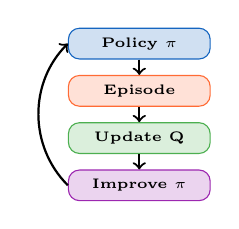
\begin{tikzpicture}[scale=0.6, every node/.style={font=\tiny}]
                        \node[rectangle, draw=mcmain, fill=mcmain!20, rounded corners=4pt, minimum width=1.8cm] (pol1) at (0,3) {\textbf{Policy $\pi$}};
                        \node[rectangle, draw=mcaccent, fill=mcaccent!20, rounded corners=4pt, minimum width=1.8cm] (ep1) at (0,2) {\textbf{Episode}};
                        \node[rectangle, draw=mcsecondary, fill=mcsecondary!20, rounded corners=4pt, minimum width=1.8cm] (q1) at (0,1) {\textbf{Update Q}};
                        \node[rectangle, draw=mceval, fill=mceval!20, rounded corners=4pt, minimum width=1.8cm] (imp1) at (0,0) {\textbf{Improve $\pi$}};

                        \draw[thick, ->] (pol1) -- (ep1);
                        \draw[thick, ->] (ep1) -- (q1);
                        \draw[thick, ->] (q1) -- (imp1);
                        \draw[thick, ->, bend left=45] (imp1.west) to (pol1.west);
                    \end{tikzpicture}
                    \end{center}

                \begin{itemize}
                    \item<2-> Same policy for \textcolor{mcmain}{\textbf{acting}} and \textcolor{mcaccent}{\textbf{learning}}
                    \item<3-> Simpler, more stable
                    \item<4-> Slower convergence
                \end{itemize}
            \end{block}
        \end{column}

        \begin{column}{0.48\textwidth}
            \begin{block}<5->{Off-Policy Monte Carlo}
                \begin{center}
                    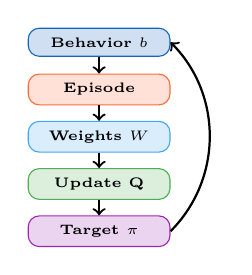
\begin{tikzpicture}[scale=0.6, every node/.style={font=\tiny}]
                        \node[rectangle, draw=mcmain, fill=mcmain!20, rounded corners=4pt, minimum width=1.8cm] (beh) at (0,3.5) {\textbf{Behavior $b$}};
                        \node[rectangle, draw=mcaccent, fill=mcaccent!20, rounded corners=4pt, minimum width=1.8cm] (ep2) at (0,2.5) {\textbf{Episode}};
                        \node[rectangle, draw=mclight, fill=mclight!20, rounded corners=4pt, minimum width=1.8cm] (weight) at (0,1.5) {\textbf{Weights $W$}};
                        \node[rectangle, draw=mcsecondary, fill=mcsecondary!20, rounded corners=4pt, minimum width=1.8cm] (q2) at (0,0.5) {\textbf{Update Q}};
                        \node[rectangle, draw=mceval, fill=mceval!20, rounded corners=4pt, minimum width=1.8cm] (tar) at (0,-0.5) {\textbf{Target $\pi$}};

                        \draw[thick, ->] (beh) -- (ep2);
                        \draw[thick, ->] (ep2) -- (weight);
                        \draw[thick, ->] (weight) -- (q2);
                        \draw[thick, ->] (q2) -- (tar);
                        \draw[thick, ->, bend right=45] (tar.east) to (beh.east);
                    \end{tikzpicture}
                \end{center}

                \begin{itemize}
                    \item<6-> Different policies for \textcolor{mcmain}{\textbf{acting}} vs \textcolor{mcaccent}{\textbf{learning}}
                    \item<7-> More complex (importance sampling)
                    \item<8-> Better exploration potential
                \end{itemize}
            \end{block}
        \end{column}
    \end{columns}
\end{frame}

% Section: Comparison and Summary
\section{Summary}

\subsection{Comparison of Methods}

\begin{frame}
    \frametitle{On-Policy vs Off-Policy: Trade-offs}

    \begin{columns}
        \begin{column}{0.5\textwidth}
            \begin{block}{On-Policy}
                \textcolor{mconpolicy}{\textbf{Advantages:}}
                \begin{itemize}
                    \item Simpler to understand
                    \item Lower variance
                    \item Faster convergence
                    \item Easier to implement
                \end{itemize}

                \vspace{0.5em}
                \textcolor{mcaccent}{\textbf{Disadvantages:}}
                \begin{itemize}
                    \item Limited to $\epsilon$-soft policies
                    \item Cannot learn deterministic optimal policy
                \end{itemize}
                \end{block}
                \end{column}
        \begin{column}{0.5\textwidth}
            \begin{block}{Off-Policy}
                \textcolor{mcoffpolicy}{\textbf{Advantages:}}
                \begin{itemize}
                    \item Can learn optimal deterministic policy
                    \item More general and powerful
                    \item Can reuse data from any policy
                \end{itemize}

                \vspace{0.5em}
                \textcolor{mcaccent}{\textbf{Disadvantages:}}
                \begin{itemize}
                    \item Higher variance
                    \item Slower convergence
                    \item More complex (importance sampling)
                \end{itemize}
            \end{block}
        \end{column}
    \end{columns}

    \begin{block}<2->{Discussion}
        \textcolor{mcactivity}{\textbf{When would you choose each approach?}}
    \end{block}
\end{frame}

\begin{frame}
    \frametitle{Practical Considerations}

    \begin{block}<1->{Implementation Tips}
        \textcolor{mcactivity}{\textbf{What should you consider when implementing Monte Carlo methods?}}
    \end{block}

    \begin{block}<2->{Choosing $\epsilon$}
        \begin{itemize}
            \item<2-> Start with $\epsilon = 0.1$ (10\% exploration)
            \item<3-> Decay $\epsilon$ over time: $\epsilon_t = \epsilon_0 / t$
            \item<4-> Balance exploration vs exploitation needs
        \end{itemize}
        \end{block}

    \begin{block}<5->{Number of Episodes}
        \begin{itemize}
            \item<5-> Monitor convergence of value estimates
            \item<6-> Plot average returns over time
            \item<7-> Consider computational budget
        \end{itemize}
        \end{block}

    \begin{block}<8->{Common Issues}
        \begin{itemize}
            \item<8-> High variance in off-policy methods
            \item<9-> Slow convergence for large state spaces
            \item<10-> Need sufficient exploration
        \end{itemize}
        \end{block}
        \end{frame}

\begin{frame}
    \frametitle{Key Takeaways}

    \begin{block}<1->{What We've Learned}
        \begin{enumerate}
            \item<1-> \textcolor{mcmain}{\textbf{Model-Free Learning:}} Can learn optimal policies without knowing environment dynamics
            \item<2-> \textcolor{mcaccent}{\textbf{Experience-Based:}} Use episodes to estimate value functions through averaging
            \item<3-> \textcolor{mcsecondary}{\textbf{Exploration is Critical:}} Must visit all state-action pairs sufficiently often
            \item<4-> \textcolor{mceval}{\textbf{Two Approaches:}} On-policy (simple) vs Off-policy (powerful)
        \end{enumerate}
    \end{block}

    \begin{block}<5->{Looking Ahead}
        \begin{itemize}
            \item<5-> Monte Carlo requires \textcolor{mcaccent}{\textbf{complete episodes}}
            \item<6-> What if episodes are very long or infinite?
            \item<7-> Next: \textcolor{mcsecondary}{\textbf{Temporal Difference Learning}} - combine MC and DP benefits
        \end{itemize}
        \end{block}
        \end{frame}

\end{document}
